\documentclass[12pt,a4paper]{report}
\setlength\textwidth{145mm}
 \setlength\topmargin{0mm}
 \setlength\headsep{0mm}
 \setlength\headheight{0mm}
 
% Přepneme na českou sazbu
\usepackage[czech]{babel}
\usepackage[IL2]{fontenc}
\usepackage{graphicx} 

%% Použité kódování znaků: obvykle latin2, cp1250 nebo utf8:
\usepackage[utf8]{inputenc}
\begin{document}


\section{Standartní implementace}
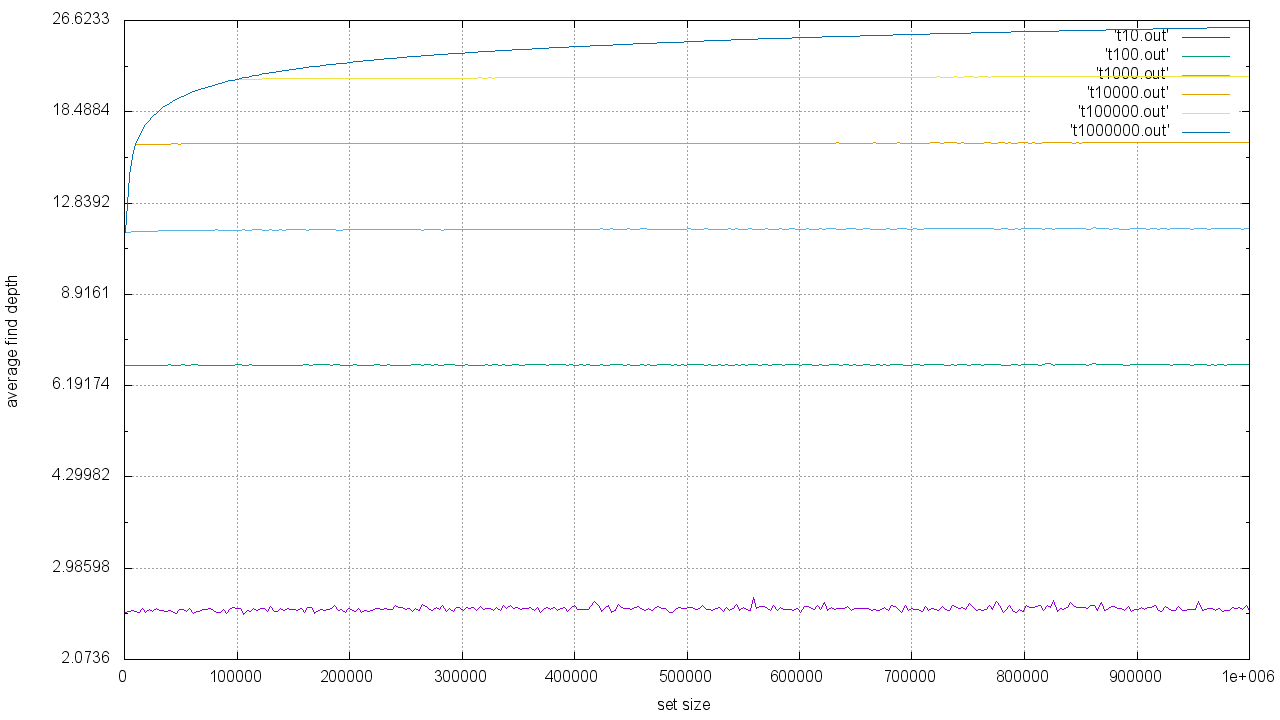
\includegraphics[width=\textwidth]{./graphs/1.png}

Na tomto grafu vidíme, že hloubky findu
se pohybují kolem stálých hodnot jen s jemným rozptylem.
Počáteční nárůst, který lze na tomto grafu sledovat pouze u t1000000,
se vyskytuje u všech grafů. (viz ./report/graphs) Tento nárůst probíhá
vždy do velikosti vyhledávané množiny a pak se ustálí.
Je také vidět, že čím menší je vyhledávaná množina, tím menší je
průměrná délka nalezení. To lze usuzovat z toho, že tato množina se
dostane blíže ke kořeni, a tak menší vyhledávané množiny musí mít
i menší hloubku vyhledání. 

\section{Naivní implementace}
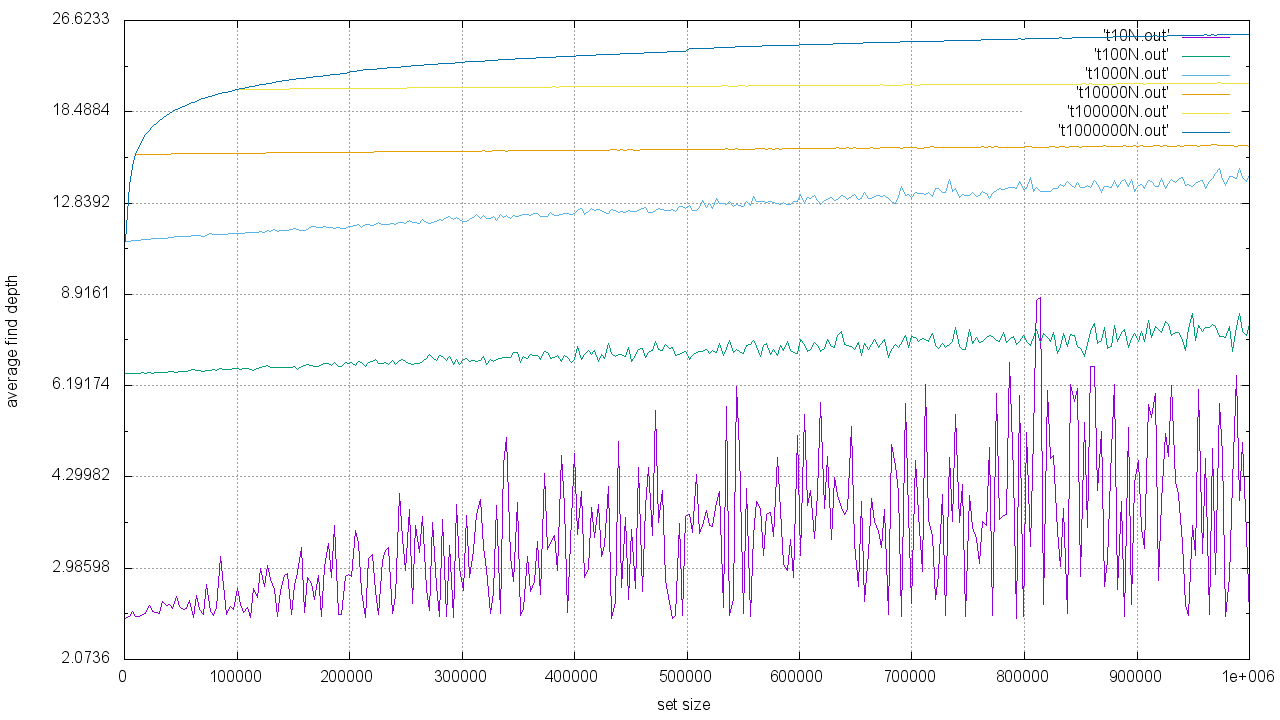
\includegraphics[width=\textwidth]{./graphs/2.png}

Pro naivní implementaci vidíme, že značně zvýšila rozptyl při 
vyhledávání. Z čehož lze usuzovat, že si tato verze při splay odsouvá
často použité vrcholy příliš rychle do hloubky. 
  
  
\section{Porovnání standartní a naivní implementace}
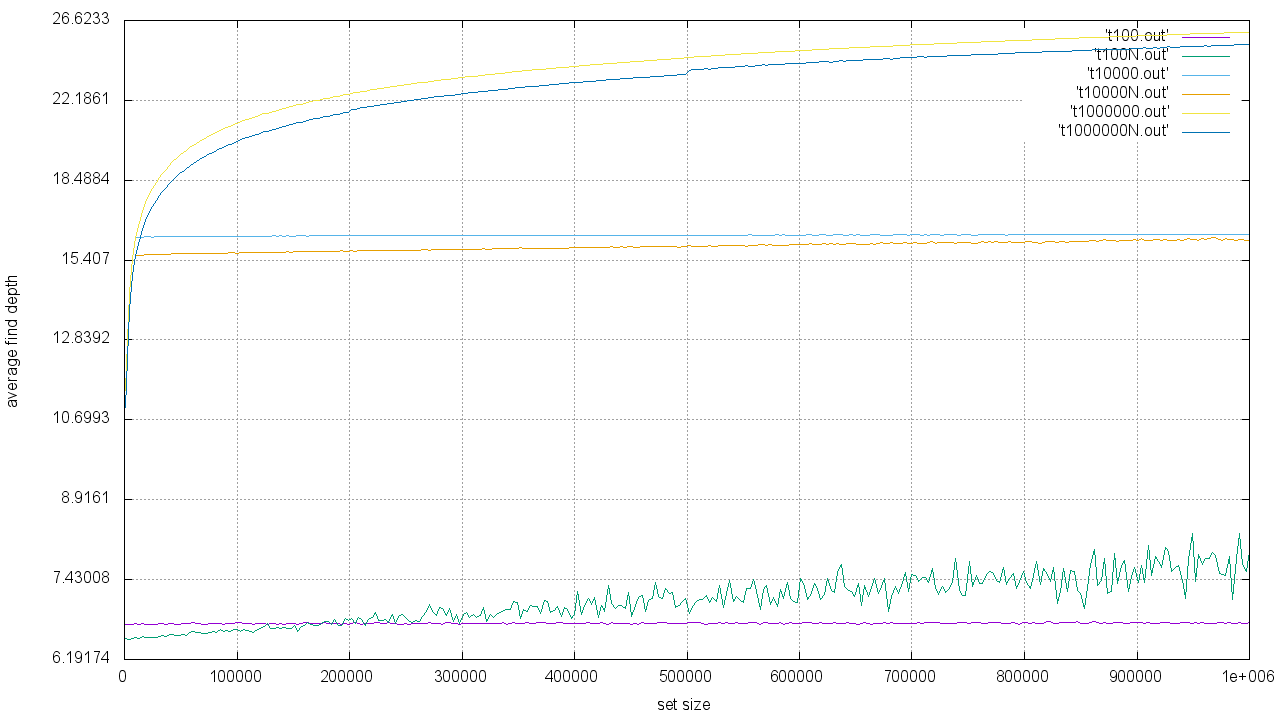
\includegraphics[width=\textwidth]{./graphs/3.png}

Je vidět, že již pro t10000 je hloubka naivních vyhledání 
o něco menší než u standartního. Nicméně narozdíl od standartní verze je
délka cesty mírně rostoucí i po dosažení počtu nalezení rovné velikosti hledané
množiny. Z toho lze usuzovat, že strom degraduje. 
  
\section{Sekvenční test}
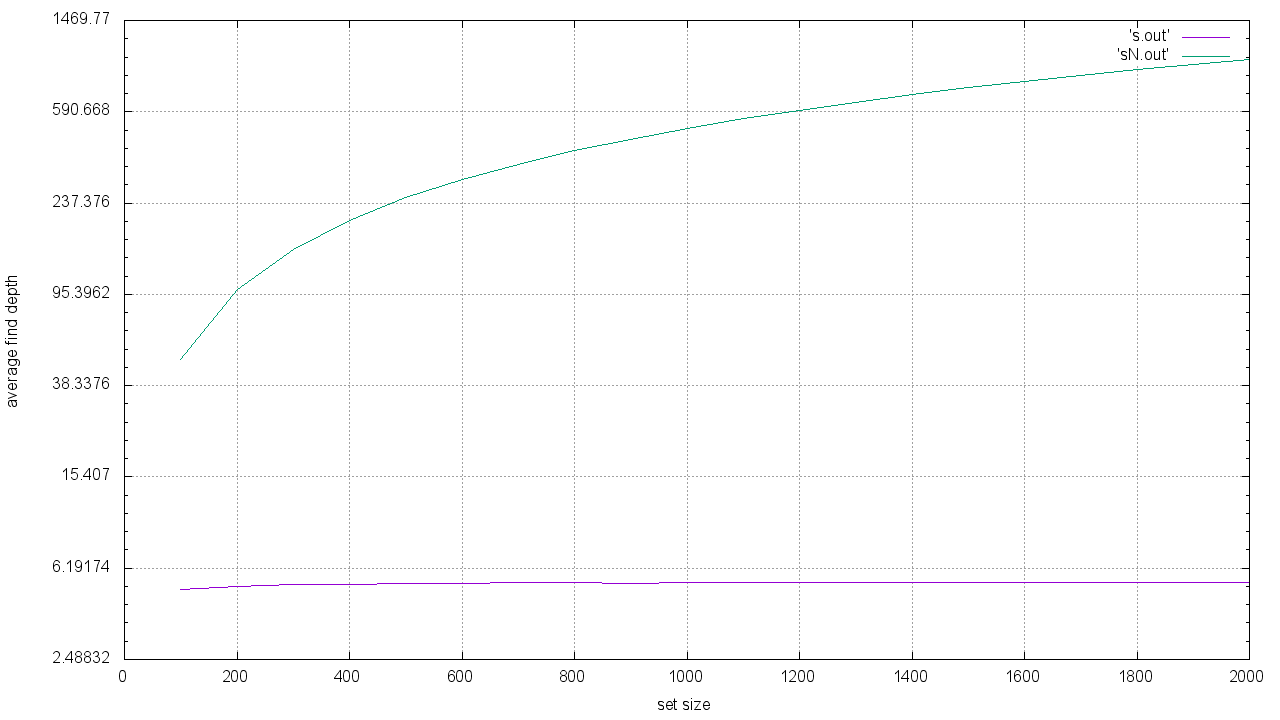
\includegraphics[width=\textwidth]{./graphs/4.png}

Zde je vidět, že naivní verze potřebuje přibližně dvakrát delší hloubku
než standartní. Také je vidět, že jednoduché rotace ,,rozbíjejí"  strom a dělají
ho vyžším. Takže stálé vyhledávání nových klíčů naivní strom rozbijí, nicméně
standartní implementace zůstává stabilní.
  
\end{document}